\chapter{Návrhové vzory Flux a Redux}

\label{kap:vzory} % id kapitoly pre prikaz ref

V tejto kapitole si povieme niečo o návrhových vzoroch Flux a Redux, ktoré sú určené na spracovávanie udalostí a globálneho stavu v aplikácii.

\section{Flux}
\label{sec:flux}
Flux \cite[Overview]{Flux} je vzor pre spravovanie dát v aplikácii. Najdôležitejším konceptom je tok informácií jedným smerom. Obsahuje štyri základné časti (zobrazené schematicky na obrázku \ref{obr:flux}). 
\begin{itemize}
\item \emph{akcie}, ktoré vytvára používateľ, prostredie (kde aplikácia beží) alebo aj časti aplikácie, 
\item \emph{dispečer} spravuje všetky vytvorené \emph{akcie}, 
\item \emph{store} reaguje na \emph{akcie} a spravuje stav aplikácie,
\item \emph{view}, ktorý vykresľuje stav aplikácie.
\end{itemize}

\subsection{Tok dát}
\begin{enumerate}
\item daný úvodný stav,
\item vykreslenie \emph{view} komponentov,
\item vznik \emph{akcie}, oznámenie \emph{akcie} dispečeru (funkcia \emph{dispatch}),
\item dispečer upozorní všetky \emph{story},
\item každý \emph{store} spracuje \emph{akciu}, prípadne zmení stav,
\item zmena v stave sa vykreslí do komponentov (2. bod).
\end{enumerate}

\begin{figure}
  \centering
    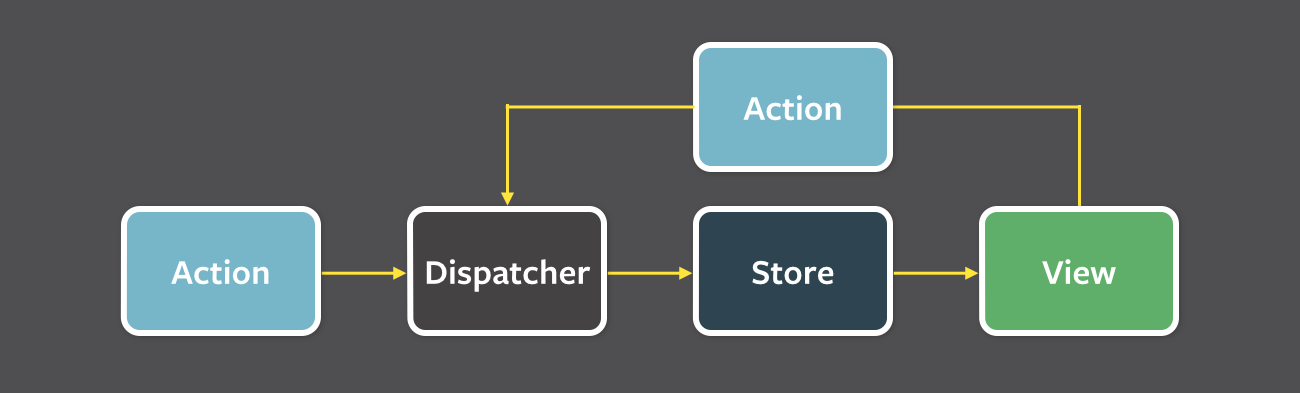
\includegraphics[width=\textwidth]{./images/flux.png}
  \caption{Flux architektúra \cite{FluxObr}}\label{obr:flux}
\end{figure}

\subsection{Dispečer (dispatcher)}
Dispečer spravuje všetky akcie vykonané v aplikácii. V celej aplikácii by mal byť len jeden. Dispečer obsahuje spätné volanie (\emph{callback}) na každý store v aplikácii. Keď sa vykoná nová akcia, dispečer pošle túto akciu všetkým storom. Sám nemusí obsahovať akúkoľvek vyššiu logiku, slúži len na distribúciu.

\subsection{Store}
Story obsahujú stav a logiku aplikácie. Store reaguje na akciu, na základe ktorej môže zmeniť stav, ktorý spravuje. Storov môže byť viac a každý upravuje nejakú podčasť dát. Každý store poskytuje dispečerovi na seba callback. Keď sa udeje nejaká akcia, bude o~tom upozornený. Na základe typu akcie sa rozhodne, či a ako bude meniť stav aplikácie (napríklad ak máme dva story Images a Texts, tak pri vytvorení akcie EditText sa pravdepodobne store Image rozhodne nič nerobiť). Po zmene stavu vytvorí udalosť, ktorou upozorní view časť, že treba prekresliť údaje.

\subsection{Akcie}
Akcie definujú internú API aplikácie. Zachytávajú možnosti interakcie s aplikáciou. Sú to jednoduché objekty s kľúčom \emph{typ} a voliteľnými pridanými informáciami. Typ akcie by nemal obsahovať žiadne implementačné detaily.

Akcie vytvára view časť (napríklad keď reagujeme na stlačenie tlačidla), server (napríklad chybová hláška počas komunikácie) alebo aj store (keď odstránime používateľa, chceme odstrániť aj všetky jeho príspevky).

\begin{lstlisting}[caption=Akcia vo Flux architektúre]
  {
  	type: 'delete-user',
  	userId: '1'
  }
\end{lstlisting}

\subsection{Views (Zobrazenie)}
View je časť návrhu, ktorá vykresľuje stav zo storu. Aby bola táto časť vždy aktuálna, musí daný view komponent počúvať na všetky udalosti od storu, ktoré hovoria o zmene relevantných dát. Ak sa zmení stav, store vytvorí udalosť a view sa prekreslí. Architektúra Flux neurčuje, ako má byť tento stav vykreslený.

\subsection{Vedľajšie efekty} 
Už sme spomínali, že jediné miesto, kde by sa mali robiť zmeny v dátach, sú story. Vedľajšie efekty často menia stav aplikácie (napríklad informácia, že sa dáta začali sťahovať zo servera, alebo sa načítali). Každý vedľajší efekt je odpoveďou na nejakú akciu. Preto tieto efekty majú veľmi často na starosti story. Ak vykonávame napríklad dotaz na server, ako spätné volanie poskytneme funkciu, ktorá vytvorí novú akciu, na~ktorú potom vie aplikácia reagovať.

Nevýhodou tohoto prístupu je, že story obsahujú aj logiku, ktorá sa deje mimo aplikácie. Často tak môžu spôsobiť (potenciálne nekonečné) narastanie počtu akcií.










\section{Redux}
Redux \cite{Redux} je popis spracovania udalostí v aplikácii. Jeho základom je Flux \ref{sec:flux}. Redux 
do~tohoto návrhu prináša prácu s čistými funkciami, ktoré spravujú stav. Oddeľuje prácu s vedĺajšími efektami do novej časti \emph{Middleware} \ref{subsec:middlewares}. Pozostáva z piatich hlavných častí (štyri zobrazené na obrázku \ref{obr:redux}):
\begin{itemize}
\item jeden \emph{store}, ktorý spravuje celý stav aplikácie,
\item \emph{reducer} - čistá funkcia, ktorá vypočíta nový stav aplikácie,
\item \emph{komponenty} vykresľujú aktuálny stav aplikácie,
\item \emph{akcie}, ktoré definujú vnútorné rozhranie aplikácie,
\item \emph{middlewares} spravujú vedľajšie efekty aplikácie.
\end{itemize}

\subsection{Tok dát}
\begin{enumerate}
\item daný úvodný stav,
\item vykreslenie \emph{komponentov},
\item vznik \emph{akcie}, dispečnutie akcie pre \emph{store},
\item \emph{reducer} na \emph{akcii} a aktuálnom stave, ktorý vráti nový stav,
\item zmena v stave sa vykreslí do \emph{komponentov} (2. bod).
\end{enumerate}

\begin{figure}
  \centering
    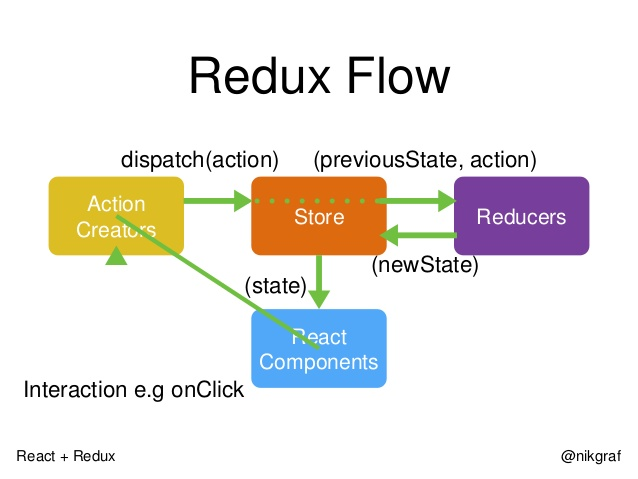
\includegraphics[width=0.8\textwidth]{./images/redux.jpg}
  \caption{Redux architektúra \cite{ReduxObr}}\label{obr:redux}
\end{figure}

\subsection{Store}
Store, správca stavu, vystupuje ako jediný zdroj pravdy v aplikácii. Všetky dáta, ktoré sú vykreslené, pochádzajú zo stavu. Teda ak poznáme tento stav, veľmi jednoducho vieme zostrojiť prostredie, v ktorom celá aplikácia beží. Rovnako v prípade chýb vieme oveľa jednoduchšie zistiť, kde chyba nastala. Tento stav je nemenný (immutable). Ak ho chceme zmeniť, musíme vytvoriť novú inštanciu, v ktorej urobíme potrebné zmeny.

Store má svoju funkciu \emph{dispatch()}, ktorá slúži na vytváranie akcií. Všetky akcie by mali byť spracované cez túto funkciu. Na tieto akcie môže store reagovať zmenou stavu.

\subsection{Komponenty}
Komponenty slúžia na vykreslenie stavu aplikácie pre používateľa. Ponúkajú rozhranie pre používateľa na komunikáciu s programom. Komponenty vieme rozdeliť na kontajnerové (\emph{Container Components}) a prezentačné (\emph{Presentational Components}).

Prezentačné komponenty iba vykresľujú dáta, ktoré dostanú. Starajú sa o~výzor aplikácie. Tieto možno používať na viacerých miestach (nadpis, tabuľka). 

Kontajnerové komponenty počúvajú na zmenu stavu. Majú na starosti, ako by mala stránka fungovať. V Redux-ovej aplikácii poskytujú rozhranie pre vytváranie akcií a~majú prístup ku funkcii dispatch.

\subsection{Akcie}
Akcia je akákoľvek udalosť, ktorá sa môže v aplikácii vyskytnúť, od stlačenia tlačidla používateľom až po chybové hlášky alebo stiahnutie dát zo servera. Na vytvorenie akcie používame funkciu \emph{dispatch}. Každá akcia musí obsahovať typ a môže voliteľne obsahovať aj prídavné dáta. Na základe tejto akcie potom reducer vypočíta nový stav.

\subsection{Reducer}
\emph{\uv{Given the same arguments, it should calculate the next state and return it. No surprises. No side effects. No API calls. No mutations. Just a calculation.}} \cite{reduxReducer}

\paragraph{}
Takmer všetka logika aplikácie sa deje v reduceroch. Reducery sú jediný objekt, ktorý môže na podnet store vypočítať nový stav aplikácie.

Reducer je čistá funkcia. Má dva argumenty, stav aplikácie a akciu, ktorá sa uskutočnila. Výstupom je nový stav. Vďaka vlastnosti, že nemá žiadne vedľajšie efekty, ju môžeme veľmi ľahko testovať.

Reducer môžeme vyskladať z viacerých menších čistých funkcií, kde každá z nich sa stará len o určitú malú časť stavu. Vďaka tomu zostáva kód prehľadný a jednoduchý. 
Pri písaní reduceru nesmieme zabúdať na to, že nový stav, ktorý vrátime, nesmie byť \uv{starý prerobený} ale musíme ho prekopírovať a dáta zmeniť až v novej inštancii.

\subsection{Perzistentné štruktúry}
Hlavnou myšlienkou reducera je, že má byť čistá funkcia. Z toho dôvodu nesmieme zmeniť vstupné parametre. Je vhodné použiť nemenné (\emph{immutable}) štruktúry. Pre väčšinu jazykov existuje natívna podpora alebo knižnica pre takéto štruktúry. Ďalšou alternatívou je striktne dodržiavať zásadu nemeniť existujúce dáta a pri zmene vrátiť novú štruktúru s aktuálnymi zmenami. Primitívne typy (string, number, boolean) sú vždy perzistentné.

\subsection{Middlewares}
\label{subsec:middlewares}
Niekedy treba robiť aj akcie, ktoré nevieme robiť lineárne, nemôžeme robiť lineárne alebo na ne len nechceme čakať. Príkladom je dopyt na server, kedy čas príchodu odpovede nezávisí od nášho programu. Vtedy môžeme použiť \emph{middleware}. Je to spoločný názov pre vedľajšie akcie. Poskytuje priestor pre rozšírenia medzi dispečnutím akcie a~notifikovaním storu (ktorý zavola reducer). Patria sem napríklad asynchrónne volania alebo volania knižníc, ktoré do vzoru Redux priamo nepatria, ale môžu s aplikáciou spolupracovať (napríklad logovanie zmien).

Asynchrónnosť môžeme implementovať viacerými spôsobmi, tie základné sú nasledujúce (predstavujeme ich s knižnicami, ktoré sú určené priamo pre návrhový vzor redux):
\begin{itemize}
  \item \emph{redux-observable} - prúd akcií, ktoré idú z dispečera, môže funkcia (middleware) zachytiť, reagovať na ne zmenou akcie alebo (často) volaním asynchrónnej funkcie. Keď funkcia vráti výsledok, môže middleware upozorniť aplikáciu o stave dobehnutej funkcie pridaním novej akcie do prúdu akcií,
  \item \emph{redux-thunk} - je založený na princípe spätných volaní. Namiesto akcie vráti funkciu, ktorá sa má vykonať. Táto funkcia bude zavolaná, a keď dobehne, vytvorí novú akciu použitím \emph{dispatch},
  \item \emph{redux-promise} - podobne ako thunk, ale namiesto spätných volaní používa promise,
  \item \emph{redux-saga} - používa generátory. Myšlienkou je mať ďalšie vlákno, ktoré spravuje vedľajšie efekty aplikácie.
\end{itemize}

V našej aplikácii používame knižnicu \emph{redux-observable}. Táto možnosť je podobná prístupu funkcie \emph{dispatchAsync}, ktorú používame vo Flux-ovej architektúre a princípu čistých funkcií zo vzoru Redux. 







\section{Porovnanie vzorov Flux a Redux}
Historicky prvý bol Flux od Facebooku. Vznikol ako náhrada modelu MVC, kde snahou Flux bolo lineárne spracovávať všetky zmeny stavu, čím sa stáva aplikácia omnoho prehľadnejšou. Po vykonaní akcie sa všetky story dozvedia o akcii a príslušné z nich na ňu reagujú.

Redux vznikol obmedzením Flux-u novými pravidlami, teda mohli by sme povedať, že je to špeciálny typ Flux-u. Kým Flux hovorí o spracovaní akcie ako takej, Redux prichádza s myšlienkou, ako meniť stav a to použitím reduceru - čistej funkcie. Použitie reducera spôsobuje, že zmena predchádzajúceho stavu na nasledujúci je plne kontrolovaná dvoma vstupnými parametrami reducera (pôvodný stav a akcia) a pri rovnakom vstupe je výstup vždy rovnaký. Vďaka tomu sa ešte viac uľahčuje testovanie prechodov medzi stavmi.

\subsection{Porovnanie častí návrhových vzorov}

\paragraph{View}
View časť je v oboch návrhoch rovnaká. V oboch je to sada komponentov, ktoré zobrazujú statické dáta a je im poskytnutá schopnosť vytvárať nové akcie. Počúvajú na zmenu dát a pri zmene sa prekreslia.

V oboch prístupoch pracujeme s virtuálnym DOM-om, teda komponenty sa prekresľujú len vtedy, ak boli zmenené (v JavaScript-ovej aplikácii sme použili knižnicu \emph{React}, v Dart-ovej aplikácii sme použili knižnicu \emph{tiles} založenú na princípe knižnice \emph{React}).

\paragraph{Akcie}
Myšlienka akcie je v oboch návrhoch rovnaká. Každá akcia je objektom, ktorý obsahuje typ a voliteľne prídavné informácie.

\paragraph{Dispatcher}
Vo Flux-e je objekt dispatcher, ktorý je jediný a idú cez neho všetky akcie. V Redux-e môže byť tento objekt vynechaný, pretože akcie sa pridávajú storu, ktorý je jediný, a ten prevezme zodpovednosť za lineárne spracovanie akcií.

\paragraph{Store}
Vo Flux-e máme jeden alebo viacero storov, v ktorých sú každý zodpovedný za nejakú logickú podčasť stavu. Každý store je upozornený o každej akcii, ktorá nastane. Na rozdiel od toho Redux obsahuje práve jeden store, ktorý je zodpovedný za celý stav.

\paragraph{Reducer}
V Reduxe tvorí jednu z hlavných častí reducer. Je zodpovedný za zmenu dát. Vo Flux-e by sme ekvivalent našli v storoch, ktoré menia dáta na základe akcií. Rozdiel je, že od reducera vyžadujeme, aby bol čistá funkcia, teda aby nezávisel na~žiadnych iných hodnotách, ako sú vstupné parametre funkcie, a nemal vedľajšie efekty. 

Reducer sa pri väčších aplikáciách zvykne rozdeliť na viacero menších reducerov, kde každý z nich spravuje celé dáta, alebo nejakú podčasť dát (napríklad ak máme dáta uložené v stromovej štruktúre, reducer môže pôsobiť na podstrome z týchto dát).

Pri storoch sme čisté funkcie nevyžadovali, keďže story potrebujú robiť napríklad dotazy na server. V Redux-e na side effects slúžia Middlewares.

\subsection{Simulovanie behu programu}
V aplikácii so vzorom Redux závisí celý stav iba od úvodného stavu a všetkých akcií, ktoré sa vytvorili v danej aplikácii. Ak máme poradie akcií, vieme celý postup zrekonštruovať. Toto je veľmi príjemná vlastnosť pri odlaďovaní aplikácie ako aj pri hľadaní chýb.
